% Options for packages loaded elsewhere
\PassOptionsToPackage{unicode}{hyperref}
\PassOptionsToPackage{hyphens}{url}
%
\documentclass[a4paper, oneside, 11pt, utf8]{article}
\usepackage{ctex}
\usepackage[top=25mm, bottom=25mm, left=20mm, right=20mm]{geometry}
\usepackage{amsmath,amssymb}
\usepackage{lmodern}
\usepackage{xcolor}
\IfFileExists{xurl.sty}{\usepackage{xurl}}{} % add URL line breaks if available
\IfFileExists{bookmark.sty}{\usepackage{bookmark}}{\usepackage{hyperref}}
\hypersetup{
  hidelinks,
  pdfcreator={LaTeX via pandoc}}
\urlstyle{same} % disable monospaced font for URLs
\usepackage{graphicx}

\author{}
\date{}

\begin{document}

\hypertarget{swap-int-and-swap-out}{%
\section{\texorpdfstring{swap int and swap out
}{swap int and swap out }}\label{swap-int-and-swap-out}}

为了实现虚拟内存

虚拟内存是连接分段和分页的关键

分段和分页是OS进行内存管理的关键

\begin{center}\rule{0.5\linewidth}{0.5pt}\end{center}

用户眼中:大而规整的内存空间 ------ 段 ------ 假象 ------ 虚拟内存

\(\downarrow\)

\textbf{映射}到物理内存

\begin{center}\rule{0.5\linewidth}{0.5pt}\end{center}

\subsection{swap in ------ 请求调用}\label{swap-in--------ux8bf7ux6c42ux8c03ux7528}

假设实际物理内存只有1G,那么,如何给用户提供一种``有4G内存的错觉''?------
内存换入

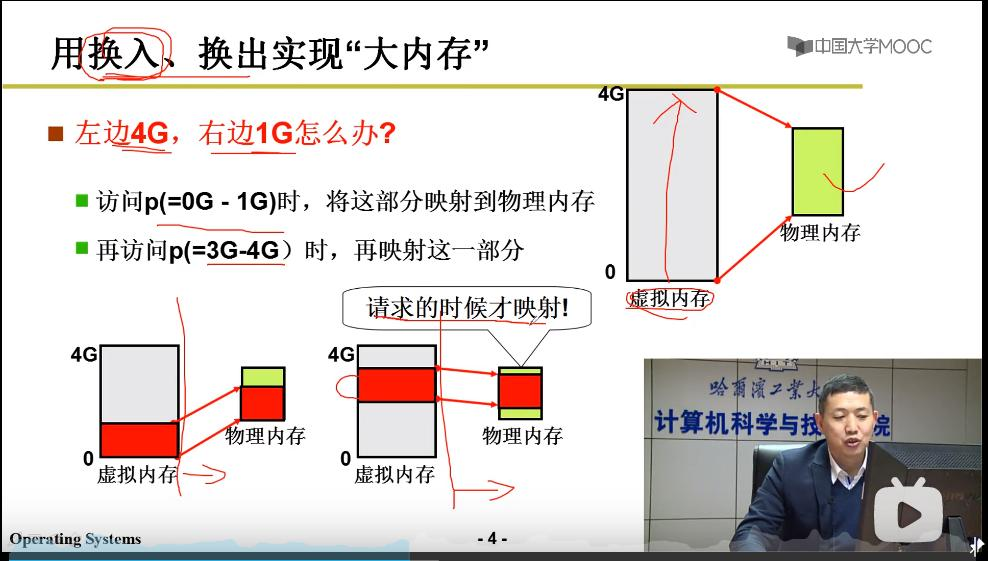
\includegraphics[scale=0.5]{/home/tony/Projects/Github/study_408/OS/class_7/img/swap_in_1G_4G.jpg}

要使用用户眼中超过实际内存大小的虚拟地址空间时,将这段虚拟内存空间
\textbf{换入} 到物理内存------请求的时候换入并建立映射 ------
请求调入页面并建立对页面的映射

\end{document}
